\chapter{Motion--Force Demonstration and Dataset Construction}
\label{chap:demonstration_collection}

\section{Teaching as a Source of Temporal Process Structure}
The purpose of teaching is to supply the motion and loading that remain unspecified by a local region. A demonstration records a tool's approach, motion through the working region, and departure together with the interaction force. This pairing supplies a temporal example for either direct replay or policy supervision. It does not include an independently measured defect-depth trajectory or a label that certifies material-removal completion.

The teaching system combines Vive tracking, a calibrated tool-pose publisher, force/torque sensing, and a RealSense RGB stream. The archived collection interface records six pose components and the first three force components. The paired data used by the evaluated models have a single RGB camera. Figure~\ref{fig:teaching_frames} shows actual frames from the selected replay episode's source, rather than a rendered apparatus or a substitute robot.

\begin{figure}[tbp]\centering
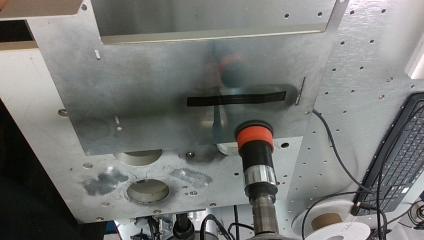
\includegraphics[width=.48\linewidth]{figures/teaching_ep29_frame000.png}\hfill
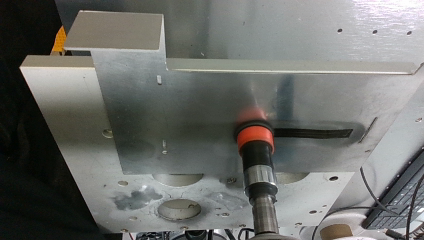
\includegraphics[width=.48\linewidth]{figures/teaching_ep29_frame085.png}\\[3pt]
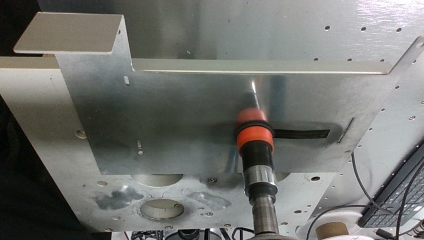
\includegraphics[width=.48\linewidth]{figures/teaching_ep29_frame150.png}\hfill
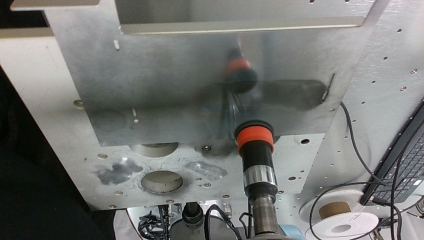
\includegraphics[width=.48\linewidth]{figures/teaching_ep29_frame400.png}
\caption[Actual teaching-camera frames]{Actual teaching-camera RGB frames associated with episode 29 at stored indices 0, 85, 150, and 400. The corresponding source is merged episode \texttt{ep\_0003}, recorded on 19 August 2026. The view shows the tool and marked plate during the recorded operation. It does not show the full tracker or sensor assembly.}
\label{fig:teaching_frames}
\end{figure}

\section{VR Registration and Tracker-to-Tool Conversion}
The recorded pose must refer to the tool rather than the tracker housing. Let \(V\) be the tracking frame, \(T\) the tracked rigid body, \(E\) the tool/TCP frame, and \(B\) the robot base. The nominal rigid coordinate chain is
\begin{equation}
 {}^BT_E(t)={}^BT_V\,{}^VT_T(t)\,{}^TT_E.
 \label{eq:demo_transfer}
\end{equation}
The fixed transforms identify the tracking world with the robot base and remove the tracker-to-tool offset. Translation is expressed in millimeters, while the final orientation is converted to a rotation vector in radians.

The implementation includes more than one rigid transform. Its calibration utilities solve the registration and tool offset, project rotations to valid rotation matrices, and support a planar correction and a bounded XY-dependent position residual. The tracker publisher converts OpenVR translation from meters to millimeters before applying the downstream calibration chain. It right-multiplies the configured spatial-angle alignment and applies the selected tool-offset convention. The published \texttt{calibrated\_pose} is the final tool pose used by the recorder; the raw tracker rotation is not substituted for it in force-axis reconstruction.

The available calibration YAML records a 47-sample fit, planar correction, and a quadratic XY residual. Its stored residual RMS changes from 4.809 to 3.179 mm for that fit. These are calibration-fit diagnostics, not an independent accuracy test of every demonstration or October execution. The source also contains a configurable final constant offset. Consequently, a single conceptual frame-chain diagram is useful for understanding the registration, while the archived parameter file remains necessary for reproducing its numerical convention.

\begin{figure}[tbp]\centering
\begin{tikzpicture}[node distance=6mm]
\node[block,text width=95mm] (a) {Vive tracker pose in tracking coordinates\\OpenVR translation converted to mm};
\node[block,text width=95mm,below=of a] (b) {VR/base registration and tracker/tool offset\\configured angle, planar, and position corrections};
\node[block,text width=95mm,below=of b] (c) {Published calibrated tool pose\\base position and rotation vector};
\node[block,text width=95mm,below=of c] (d) {Stain-centered learning pose\\subtract center; retain teaching direction, Z, and orientation};
\node[block,text width=95mm,below=of d] (e) {Optional direction transfer at inference\\align live XY and image with the teaching reference};
\node[block,text width=95mm,below=of e] (f) {Restore generated XY to the live task\\inverse rotation, then center addition};
\draw[link](a)--(b);\draw[link](b)--(c);\draw[link](c)--(d);
\draw[link](d)--(e);\draw[link](e)--(f);
\end{tikzpicture}
\caption[Coordinate-processing and direction-transfer chain]{Implemented coordinate-processing roles, shown as an editable conceptual diagram. Calibration establishes the tool pose; center-relative learning and optional direction alignment register the local movement pattern. The last two boxes show the inference transfer in Equations~\eqref{eq:stain_canonical_observation} and~\eqref{eq:stain_canonical_action}, disabled in E1/E2. Only XY positions are rotated; tool orientation and force channels retain their conventions.}
\label{fig:demo_transfer}
\end{figure}

\section{Synchronized Recording and the Meaning of Time}
The source merged HDF5 identifies its schema as multimodal synchronized recording, its master as camera 0, and its clock as subscriber-receive Unix time. The camera observation supplies the common sample time. Pose and force are associated through receive-time buffers, with a recorded maximum synchronization error parameter of 0.05 s. The archive retains the source times, interpolation indicators, and pose/force synchronization errors for each paired sample.

These timestamps describe software receipt and pairing. They are not hardware exposure timestamps or the original force-sensor acquisition times. Their value is that the construction of a paired sample is explicit and can be inspected. Their limitation is that transport delay and sensor latency cannot be removed simply by assigning all signals to one image time.

The representative source episode records a nominal 30 Hz grid, 443 paired frames, and the original \texttt{sample\_time\_unix} array. The compact learning file retains the paired images and signals but not that full time array. For the replay baseline and the teaching plots, the source episode is recovered using the compact file's \texttt{source\_h5} and \texttt{source\_episode} attributes. This preserves the actual paired time axis instead of reconstructing it solely from the nominal rate.

\section{Signal Stages and Force Processing}
The word raw depends on where a signal enters the pipeline. The recorder's \texttt{raw\_ft} is already a decoded and published measurement after the configured sign, startup-zero, and gravity-processing path. It is raw relative to the recorder's offline filter. It is not an uncorrected packet from the force sensor.

The teaching publisher applies its configured sensor decoding and sign convention, startup mean zeroing, selected publisher filtering, and delta-gravity compensation before publishing the wrench. The recorder then applies native-axis force filtering. In the representative archived episode, the force filter is an exponential moving average with \(\alpha=0.2\),
\begin{equation}
 \bar f_k=\alpha f_k+(1-\alpha)\bar f_{k-1}.
 \label{eq:force_ema}
\end{equation}
The stored pose is processed through the existing Hampel and difference-regularized smoothing pipeline. The archived episode reports no pose EMA, no approach slowdown, and retiming factor one. These are properties of the selected recorded episode; optional processing branches in the current recorder are not assumed to have been active.

\begin{table}[tbp]\centering\small
\caption[Teaching and learning signal stages]{Teaching and learning signal stages. Normalization changes scale for the network; it does not perform physical calibration.}
\label{tab:signal_stages}
\begin{tabularx}{\textwidth}{P{0.25\textwidth}X}
\toprule Stage & Meaning and use \\ \midrule
Published / recorder raw & Decoded and compensated force paired with calibrated pose; preserved as \texttt{raw\_ft} and \texttt{raw\_position}. \\
Filtered recording & Existing pose processing and force EMA; paired images and source-time mapping retained. \\
Learning cleanup & Derived force fields modified by the specified native-axis cleanup; pose and RGB preserved. \\
Normalized tensors & Training-split bounds map pose and force channels to the network scale. B then masks its force-conditioning tensors. \\
\bottomrule
\end{tabularx}
\end{table}

The 12 October force-cleanup dataset is a derived copy. It preserves the 42 episodes' images and pose fields, sets negative native \(F_z\) values to zero, and sets all three force components to zero where the associated stored \(z>175\) mm. Signed \(F_x,F_y\) remain unchanged in the other samples. The same rules apply to observation and action force fields. This height rule is an offline preprocessing convention tied to the stored coordinate system, not a new real-time contact detector or an estimate of material-removal depth.

Figure~\ref{fig:force_processing} shows these stages for the representative episode. Learning nonnegative targets does not impose a nonnegative output constraint on the generator. The archived model checks include negative unconditioned force predictions in some chunks; the runtime must therefore be described from its actual gating and command-processing code, rather than by assuming cleanup enforces a physical output bound.

\figfull{force_processing.pdf}{Actual force-processing stages for teaching episode 29. The upper panel compares post-publisher recorder raw force, offline EMA, and the learning cleanup in native axes. The lower panel rotates the complete cleanup force vector to robot-base axes using its paired tool orientation. These are different signal stages; none is a new physical calibration.}{fig:force_processing}

\section{Force Frames and Common-Axis Analysis}
The existing force correspondence analysis supplies a resolved relation between teaching published axes and the calibrated tool frame:
\begin{equation}
 R_{E\leftarrow\mathrm{pub}}=I,\qquad
 f_B(t)=R_{B\leftarrow E}(t)\,f_{\mathrm{pub,processed}}(t).
 \label{eq:normal_force_projection}
\end{equation}
The second relation is posture dependent. All three force components are rotated using the calibrated tool rotation. Sign, zero, and gravity corrections are already present in the published vector and are not applied again. Translating the XY task origin does not rotate force.

Robot feedback follows a different processing chain: startup zeroing, the archived moving-average stage, a fixed sensor-to-TCP rotation, TCP gravity correction, and TCP-to-base rotation before publication and copying into the current-force topic. The executor's recorded force is therefore already in robot-base axes. Re-rotating that CSV would be incorrect.

Common-axis reconstruction makes the recorded teaching distribution and measured robot-base component comparable for an empirical force-exposure statistic. It does not recover an unlogged controller-applied target or establish a force-tracking error. It also does not imply that training tensors were retrospectively rotated. The evaluated dataset keeps native teaching force, while the inference adapter reads the selected robot-force components directly before normalization. This numerical input convention is retained when reporting the actual evaluated implementation. A common-frame policy-training ablation was not performed.

\section{Relative Coordinates, Episodes, and Data Partitions}
The compact representation subtracts the stored stain center from observation and action XY positions, leaving Z and orientation unchanged. Learning this local pattern removes absolute XY placement from the pose supervision. The selected dataset is labeled single-direction, 90-degree, and explicitly records \texttt{rotation\_aligned=false}. This attribute describes the saved training data; it does not mean that the implementation lacks direction transfer. The separate inference adapter in Section~\ref{sec:stain_relative_generalization} aligns live positions and images to a configured teaching direction and inversely restores generated XY. E1/E2 explicitly disable that adapter, so their results do not quantify its transfer performance. Some upstream files also record episode-specific XYZ corrections, which are preprocessing transformations rather than separate generalization tests.

The evaluated A/B/C models share 42 unique episodes. The optimization partition contains 38 episodes; validation contains episodes 35, 39, 22, and 37. The checkpoint normalizer files reproduce this episode-level partition. All windows from an episode remain in its assigned partition, avoiding overlap of windows from one episode across optimization and validation. This does not establish independence by operator, material, specimen, or collection session. No separate held-out demonstration-test split is claimed.

\figfull{dataset_split.pdf}{Stored lengths of all 42 episodes used by the force-cleanup models. Orange identifies the four validation episodes. The partition is made before window sampling; repeated windows are not independent demonstrations.}{fig:dataset_split}

The loader draws 50 start indices per episode and constructs a 128-step future sequence. End-of-episode padding repeats the final action and masks padded positions out of the loss. Force history includes the current sample and the preceding samples up to a length of 30; a short initial history is padded on the left with the first available value. Start sampling is resampled across training epochs. Its existing phase sampler upweights the one-second precontact period by five relative to free and contact periods, using the recorded force thresholds of 3.0 and 1.2 N. The offline sampler uses this force-derived phase information for all three conditions, including A. A's policy still receives no force observation or force target.

Normalization bounds are computed from optimization-training episodes only. For channel \(d\), the implemented min--max mapping is
\begin{equation}
 \mathcal N_d(x)=2\frac{x-m_d}{\max(M_d-m_d,\epsilon)}-1,
 \label{eq:minmax_normalization}
\end{equation}
where \(m_d,M_d\) are the stored training bounds and \(\epsilon\) is the numerical denominator floor. State and action bounds are stored separately; force history uses the state-force bounds. Normalization does not force all future online values to lie within the training range.

\section{A Representative Motion--Force Pairing}
Episode 29 is used to explain the temporal representation because it is the operator-selected replay source, rather than an episode chosen for low error. Figure~\ref{fig:teaching_motion_force} presents its actual position and force history. The transition from approach to loaded movement and then rising motion gives a structured association between location, loading, and time. Replay uses that association directly; learning uses many such future windows as supervision.

\figfull{teaching_motion_force.pdf}{Teaching episode 29 on the original paired source-time axis. XY is task relative, Z remains in the stored absolute convention, and force is the native-axis cleanup signal. The 175 mm line is the offline cleanup boundary. The curves are not a desired-versus-measured robot force-tracking comparison.}{fig:teaching_motion_force}

The force action derives from measured teaching interaction, not an independently recorded human command. Physical equivalence must be assessed from robot measurements because the mechanics and controller differ.
